\documentclass[aspectratio=169,unicode,dvipdfmx,14pt]{beamer}

\usepackage{url}
\usepackage{bm}
\usepackage{amsmath}
\usepackage{amssymb}
\usepackage{graphicx}
\usepackage[absolute,overlay]{textpos}
\usepackage{hyperref}
\usepackage{listings}

\usefonttheme[onlymath]{serif}

\DeclareMathOperator*{\argmax}{argmax}

\hypersetup{
	setpagesize=false,
	bookmarksnumbered=true,%
	bookmarksopen=true,%
	colorlinks=true,%
	linkcolor=blue,
	citecolor=red,
}

\newcommand\FontMath{\fontsize{10}{12}\selectfont}
\renewcommand{\baselinestretch}{1.3}
\renewcommand{\familydefault}{\sfdefault}
\renewcommand{\kanjifamilydefault}{\gtdefault}
\usepackage[deluxe, expert]{otf}

\setbeamertemplate{navigation symbols}{}
\setbeamertemplate{footline}[frame number]
\setbeamerfont{footline}{size={\fontsize{15}{15}}}

\setbeamerfont{author}{size=\Large}
\setbeamerfont{institute}{size=\normalsize\itshape}
\setbeamerfont{title}{size=\huge}
\setbeamerfont{subtitle}{size=\LARGE\normalfont\slshape}


\title{ \\正規分布を使った\\ベイズ的モデリング}
\author{\texorpdfstring{正田 備也\newline\href{mailto:masada@rikkyo.ac.jp}{masada@rikkyo.ac.jp}}{正田 備也}}
\date{}

\begin{document}

\begin{frame}
\titlepage
\end{frame}

\section{正規分布の復習}

\begin{frame}\frametitle{Contents}
\Large \tableofcontents[currentsection]
\end{frame}

\begin{frame}{単変量正規分布}
\begin{itemize}
\item 単変量正規分布は、$\mathbb{R}=(-\infty,\infty)$上に定義される
\item 単変量正規分布のパラメータは、平均$\mu$と標準偏差$\sigma$
\begin{itemize}
\item 平均$\mu$、標準偏差$\sigma$の単変量正規分布を、以下、$\mathcal{N}(\mu,\sigma^2)$と書く
\item 確率変数$x$が$\mathcal{N}(\mu,\sigma^2)$に従うことを、以下、$x\sim\mathcal{N}(\mu,\sigma^2)$と書く
\end{itemize}
\item 単変量正規分布$x\sim\mathcal{N}(\mu,\sigma^2)$の確率密度関数:
\begin{align}
p(x;\mu,\sigma) = \frac{1}{\sqrt{2\pi\sigma^2}}\exp\Big( - \frac{(x - \mu)^2}{2\sigma^2} \Big)
\end{align}
\end{itemize}
\end{frame}

\begin{frame}{多変量正規分布}
\begin{itemize}
\item パラメータ:
\begin{itemize}
\item 平均ベクトル
$\bm{\mu} = \begin{bmatrix} \mu_1 \\ \vdots \\ \mu_d \end{bmatrix}$
\item 分散共分散行列
$\bm{\Sigma} = \begin{bmatrix} \sigma_{11} & \cdots & \sigma_{1d} \\ 
\vdots & \ddots & \vdots \\
\sigma_{1d} & \cdots & \sigma_{dd} \end{bmatrix}$
(ただし$\Sigma$は正定値行列)
\end{itemize}
\item 確率密度関数(ただし$| \bm{\Sigma} | \equiv \mbox{det}\bm{\Sigma}$):
\begin{align}
p(\bm{x};\bm{\mu},\bm{\Sigma}) = \frac{1}{\sqrt{(2\pi)^d|\bm{\Sigma}|}}\exp\bigg\{ - \frac{(\bm{x} - \bm{\mu})^\intercal \bm{\Sigma}^{-1} (\bm{x} -\bm{\mu})}{2} \bigg\}
\end{align}
\end{itemize}
\end{frame}

\begin{frame}{多変量正規分布の実際}
\begin{itemize}
\item 実際には共分散行列を対角行列と仮定することも多い
\begin{itemize}
\item $\bm{\Sigma}$の逆行列の計算が、しばしば数値計算的に難しい
\begin{itemize}
\item 例えば、変分オートエンコーダvariational autoencoderや拡散確率モデルdiffusion probabilistic modelでも共分散行列が対角行列だと仮定する
\end{itemize}
\end{itemize}
\item このとき密度関数は単変量正規分布の密度関数の積となる:
\begin{align}
p(\bm{x};\bm{\mu},\bm{\Sigma}) & = \frac{1}{\sqrt{(2\pi)^d|\bm{\Sigma}|}}\exp\bigg\{ - \frac{(\bm{x} - \bm{\mu})^\intercal \bm{\Sigma}^{-1} (\bm{x} -\bm{\mu})}{2} \bigg\}
\notag \\ & =
\prod_{j=1}^d \frac{1}{\sqrt{2\pi\sigma_j^2}}\exp\Big( - \frac{(x_j - \mu_j)^2}{2\sigma_j^2} \Big)
\end{align}
\end{itemize}
\end{frame}

\begin{frame}{単変量正規分布に従う観測データの尤度}
\begin{itemize}
\item 与えられている観測データを$\mathcal{D}=\{x_1,\ldots,x_N\}$とする
\begin{itemize}
\item 各$x_i$は、$-\infty < x_i < \infty$を満たす実数値とする
\end{itemize}
\item 各観測データ$x_i$を、同じ正規分布$\mathcal{N}(\mu,\sigma)$に独立にしたがうものとしてモデル化することにする(つまりi.i.d.を仮定)
\item このとき、データセット$\mathcal{D}$の尤度は以下のように$\mu$と$\sigma$の関数として書くことができる:
\begin{align}
p(\mathcal{D};\mu,\sigma)=\prod_{i=1}^N p(x_i;\mu,\sigma)
=\prod_{i=1}^N \frac{1}{\sqrt{2\pi\sigma^2}}\exp\bigg( - \frac{(x_i - \mu)^2}{2\sigma^2}\bigg)
\label{eq:normal_LL}
\end{align}
\end{itemize}
\end{frame}


\begin{frame}{単変量正規分布の最尤推定}
\begin{itemize}
\item 式\eqref{eq:normal_LL}より、観測データ$\mathcal{D}=\{ x_1, \ldots, x_N \}$の対数尤度は
\begin{align}
\ln p(\mathcal{D};\mu,\sigma)
= - \frac{N}{2}\ln(2\pi\sigma^2) - \sum_{i=1}^N \frac{(x_i - \mu)^2}{2\sigma^2}
\end{align}
\item この対数尤度を最大化する$\mu$と$\sigma$を求めると
\begin{align}
\hat{\mu} = \frac{\sum_i x_i}{N} = \bar{x} \mbox{ , \ }
\hat{\sigma}^2 = \frac{\sum_i (x_i - \bar{x})^2}{N}
\end{align}
\end{itemize}
\end{frame}

\begin{frame}{多変量正規分布の最尤推定 (1/2)}
\begin{itemize}
\item 観測データ$\mathcal{D}=\{ \bm{x}_1, \ldots, \bm{x}_N \}, \bm{x}_i \in \mathbb{R}^d$の対数尤度は
\end{itemize}
\begin{align}
p(\mathcal{D};\bm{\mu},\bm{\Sigma})
=
\prod_{i=1}^N \frac{1}{\sqrt{(2\pi)^d|\bm{\Sigma}|}}
\exp\bigg[ - \frac{1}{2} (\bm{x}_i - \bm{\mu})^\intercal \bm{\Sigma}^{-1} (\bm{x}_i - \bm{\mu}) \bigg]
\end{align}
\begin{itemize}
\item この対数尤度を最大化する$\bm{\mu}$と$\bm{\Sigma}$を求めると
\begin{align}
\hat{\bm{\mu}} = \frac{\sum_i \bm{x}_i}{N} = \bar{\bm{x}} \mbox{ , \ }
\hat{\bm{\Sigma}} = \frac{1}{N}\sum_i (\bm{x}_i - \bm{\mu}) (\bm{x}_i - \bm{\mu})^\intercal
\end{align}
\end{itemize}
\end{frame}


\begin{frame}{多変量正規分布の最尤推定 (2/2)}
\begin{itemize}
\item 共分散行列が対角行列だと仮定する
\item 観測データ$\mathcal{D}=\{ \bm{x}_1, \ldots, \bm{x}_N \}, \bm{x}_i \in \mathbb{R}^d$の対数尤度は
\end{itemize}
\begin{align}
\ln p(\mathcal{D};\bm{\mu},\bm{\Sigma})
= -\frac{N}{2}\sum_{j=1}^d \ln(2\pi\sigma_j^2) - \sum_{i=1}^N \sum_{j=1}^d \frac{(x_{i,j} - \mu_j)^2}{2\sigma_j^2}
\end{align}
\begin{itemize}
\item この対数尤度を最大化する$\bm{\mu}$と$\bm{\Sigma}$を求めると
\begin{align}
\hat{\mu}_j = \frac{\sum_i x_{i,j}}{N} = \bar{x}_j \mbox{ , \ }
\hat{\sigma}_j^2 = \frac{\sum_i (x_{i,j} - \bar{x}_j)^2}{N}
\end{align}
\end{itemize}
\end{frame}


\section{正規分布を使ったベイズ的モデリング}

\begin{frame}\frametitle{Contents}
\Large \tableofcontents[currentsection]
\end{frame}

\begin{frame}{ベイズ的なモデリングとは}
\begin{itemize}
\item 統計モデルは観測データの不確かさuncertaintyを表現する
\item だが、ベイズ的な統計モデリングでは、観測データをもとにして統計モデルのパラメータを決めること自体も不確かさuncertaintyをはらんでいると考える
\item そこで、パラメータも確率変数とみなし、パラメータも確率分布にしたがっているものとしてモデリングする
\item そこで導入されるのが事前分布である
\item 事前分布はパラメータがしたがう確率分布として導入される
\end{itemize}
\end{frame}

\begin{frame}{単変量正規分布を使うベイズ的モデリング(1)}
\begin{itemize}
\item 観測データ$\mathcal{D}=\{x_1,\ldots,x_N\}$の尤度は$p(\mathcal{D}|\mu,\sigma)$
\begin{itemize}
\item 事前分布を使わないときは$p(\mathcal{D};\mu,\sigma)$と書いていた
\item ベイズ的モデリングでは、$p(\mathcal{D}|\mu,\sigma)$と、条件確率として書く
\item 観測変数$\bm{x}$だけでなく、$\mu$と$\sigma$も確率変数となるからである
\end{itemize}
\item まず、$\mu$についてだけ、それがしたがう事前分布を導入する
\begin{itemize}
\item つまり、$\sigma$は自由パラメータのままとする
\end{itemize}
\item このとき、正規分布が共役事前分布となる
\begin{itemize}
\item このことを次の2枚のスライドで示す
\end{itemize}
\item $\mu$の事前分布を$\mathcal{N}(\mu_0,\sigma_0)$とする
\end{itemize}
\end{frame}

\begin{frame}{共役事前分布としての正規分布}
\FontMath
\vspace{-.2in}
\begin{align}
& p(\mathcal{D}|\mu,\sigma)p(\mu;\mu_0,\sigma_0)
= \prod_{i=1}^N \frac{1}{\sqrt{2\pi}\sigma}\exp\bigg[ - \frac{  (x_i - \mu)^2 }{2\sigma^2} \bigg]
\times \frac{1}{\sqrt{2\pi}\sigma_0} \exp \bigg[ - \frac{  (\mu - \mu_0)^2  }{2\sigma_0^2} \bigg]
\notag \\ & =
\frac{1}{(\sqrt{2\pi})^N\sigma^N}\exp\bigg[ - \frac{  \sum_i (x_i - \mu)^2 }{2\sigma^2} \bigg]
\times \frac{1}{\sqrt{2\pi}\sigma_0} \exp \bigg[ - \frac{  (\mu - \mu_0)^2  }{2\sigma_0^2} \bigg]
\notag \\ & =
\frac{1}{(\sqrt{2\pi})^N\sigma^N}\exp\bigg[ - \frac{  N\mu^2 - 2\sum_i x_i \mu + \sum_i x_i^2 }{2\sigma^2} \bigg]
\times \frac{1}{\sqrt{2\pi}\sigma_0} \exp \bigg[ - \frac{  \mu^2 - 2\mu_0\mu + \mu_0^2  }{2\sigma_0^2} \bigg]
\notag \\ & =
\frac{1}{(\sqrt{2\pi})^N\sigma^N\sigma_0}
\exp\bigg[ 
- \Big( \frac{N}{2\sigma^2} + \frac{1}{2\sigma_0^2} \Big) \mu^2 
+ 2 \Big( \frac{ \sum_i x_i}{2\sigma^2} + \frac{\mu_0}{2\sigma_0^2} \Big) \mu 
- \frac{ \sum_i x_i^2}{2\sigma^2} - \frac{\mu_0^2}{2\sigma_0^2} \bigg]
\end{align}
よって
\begin{align}
p(\mu | \mathcal{D}; \mu_0, \sigma_0)
\propto
\exp\bigg[ 
- \Big( \frac{N}{2\sigma^2} + \frac{1}{2\sigma_0^2} \Big) \mu^2 
+ 2 \Big( \frac{ \sum_i x_i}{2\sigma^2} + \frac{\mu_0}{2\sigma_0^2} \Big) \mu \bigg]
\end{align}
指数関数の中身に注目すると・・・
\end{frame}

\begin{frame}
\FontMath
\begin{align}
& \Big( \frac{N}{2\sigma^2} + \frac{1}{2\sigma_0^2} \Big) \mu^2 
- 2 \Big( \frac{ \sum_i x_i}{2\sigma^2} + \frac{\mu_0}{2\sigma_0^2} \Big) \mu 
=
\frac{N\sigma_0^2 + \sigma^2}{2\sigma^2\sigma_0^2} \bigg(
\mu^2 
-  2\frac{ N \sigma_0^2 \bar{x}  + \sigma^2 \mu_0 }{ N\sigma_0^2 + \sigma^2 } \mu \bigg)
\notag \\ & =
\frac{N\sigma_0^2 + \sigma^2}{2\sigma^2\sigma_0^2}
\bigg( \mu - \frac{ N \sigma_0^2 \bar{x}  + \sigma^2 \mu_0 }{ N\sigma_0^2 + \sigma^2 } \bigg)^2
+ const.
\end{align}
以上より、
\begin{align}
p(\mu | \mathcal{D}; \mu_0, \sigma_0)
\propto \exp\bigg[
- \frac{N\sigma_0^2 + \sigma^2}{2\sigma^2\sigma_0^2}
\bigg( \mu - \frac{ N \sigma_0^2 \bar{x}  + \sigma^2 \mu_0 }{ N\sigma_0^2 + \sigma^2 } \bigg)^2
\bigg]
\end{align}
よって、事後分布$p(\mu | \mathcal{D}; \mu_0, \sigma_0)$は、
平均が$\frac{ N \sigma_0^2 \bar{x}  + \sigma^2 \mu_0 }{ N\sigma_0^2 + \sigma^2 }$、
分散が$\frac{\sigma^2\sigma_0^2}{N\sigma_0^2 + \sigma^2}$の正規分布であることが分かる。
\begin{itemize}
\item 平均$\frac{ N \sigma_0^2 \bar{x}  + \sigma^2 \mu_0 }{ N\sigma_0^2 + \sigma^2 }$は、
標本平均と事前分布の平均$\mu_0$を$\frac{N}{\sigma^2}$対$\frac{1}{\sigma_0^2}$の割合で混ぜたもの
\item 分散$\frac{\sigma^2\sigma_0^2}{N\sigma_0^2 + \sigma^2}$の逆数は、$\frac{N}{\sigma^2}$と$\frac{1}{\sigma_0^2}$の和になっている
\item なお、分散の逆数を精度 precision という
\end{itemize}
\end{frame}

\begin{frame}{単変量正規分布を使うベイズ的モデリング(2)}
\begin{itemize}
\item 観測データ$\mathcal{D}=\{x_1,\ldots,x_N\}$の尤度は$p(\mathcal{D}|\mu,\sigma)$
\item 今度は、$\mu$と$\sigma^2$の両方について事前分布を導入する
\item ただし、分散$\sigma^2$については、その逆数である精度$\tau \equiv \sigma^{-2}$がしたがう事前分布を導入する
\item このとき、正規ガンマ分布normal-gamma distributionが共役事前分布となる
\item 正規ガンマ分布の確率密度関数は
\begin{align}
p(\mu, \tau ; \mu_0, \lambda_0, \alpha, \beta)
= \frac{\beta^\alpha\sqrt{\lambda_0}}{\Gamma(\alpha)\sqrt{2\pi}}
\tau^{\alpha-\frac{1}{2}}e^{-\beta\tau}e^{-\frac{\lambda_0\tau(\mu - \mu_0)^2}{2}}
\end{align}
\end{itemize}
\end{frame}

\begin{frame}{ガンマ分布}
\begin{itemize}
\item ガンマ分布は非負実数$[0,\infty)$上に定義される確率分布
\item パラメータ
\begin{itemize}
\item shapeパラメータ$\alpha$
\item rateパラメータ$\beta$
\end{itemize}
\item ガンマ分布の確率密度関数は
\item[] \
\begin{align}
p(x;\alpha,\beta)=\frac{\beta^\alpha}{\Gamma(\alpha)}x^{\alpha-1}e^{-\beta x}
\end{align}
\end{itemize}
\begin{textblock*}{0.4\linewidth}(260pt, 70pt)
    \centering
    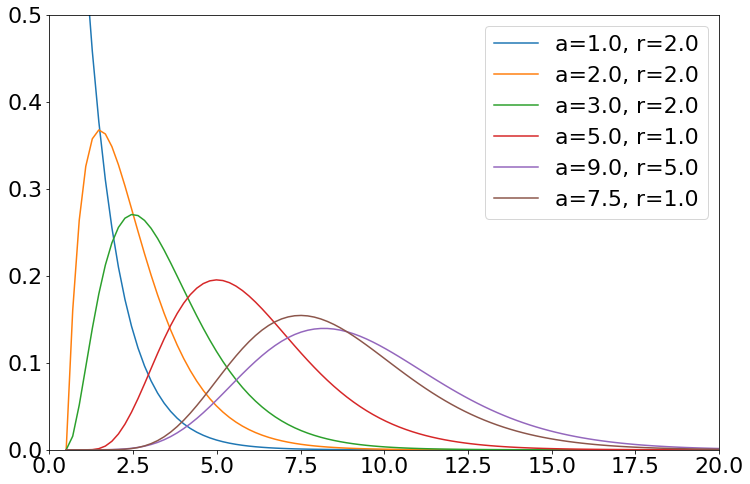
\includegraphics[width=1.1\linewidth]{gamma_dist.png}
\end{textblock*}
\end{frame}

\begin{frame}{正規ガンマ分布の密度関数の見方}
\FontMath
$\mu$を周辺化する(積分消去する)と
\begin{align}
& p(\tau ; \mu_0, \lambda_0, \alpha, \beta) = \int_{-\infty}^\infty p(\mu, \tau ; \mu_0, \lambda_0, \alpha, \beta) d\mu
= \frac{\beta^\alpha\sqrt{\lambda_0}}{\Gamma(\alpha)\sqrt{2\pi}}
\tau^{\alpha-\frac{1}{2}}e^{-\beta\tau}
\int_{-\infty}^\infty e^{-\frac{\lambda_0\tau(\mu - \mu_0)^2}{2}} d\mu
\notag \\ &
= \frac{\beta^\alpha\sqrt{\lambda_0}}{\Gamma(\alpha)\sqrt{2\pi}}
\tau^{\alpha-\frac{1}{2}}e^{-\beta\tau}
\sqrt{ \frac{2\pi}{\lambda_0\tau} }
= \frac{\beta^\alpha}{\Gamma(\alpha)}
\tau^{\alpha-1}e^{-\beta\tau}
\end{align}
ガンマ分布を得る。よって、条件付き密度関数$p(\mu | \tau ; \mu_0, \lambda_0, \alpha, \beta)$は
\begin{align}
& p(\mu | \tau ; \mu_0, \lambda_0, \alpha, \beta)
= \frac{ p(\mu, \tau ; \mu_0, \lambda_0, \alpha, \beta) }{ p(\tau ; \mu_0, \lambda_0, \alpha, \beta) }
\notag \\ &
= \frac{ \frac{\beta^\alpha\sqrt{\lambda_0}}{\Gamma(\alpha)\sqrt{2\pi}}
\tau^{\alpha-\frac{1}{2}}e^{-\beta\tau}e^{-\frac{\lambda_0\tau(\mu - \mu_0)^2}{2}} }
{ \frac{\beta^\alpha}{\Gamma(\alpha)}
\tau^{\alpha-1}e^{-\beta\tau} }
= \sqrt{ \frac{ \lambda_0\tau }{ 2\pi } } \exp\bigg( - \frac{\lambda_0\tau(\mu - \mu_0)^2}{2} \bigg)
\end{align}
と、正規分布になる。つまり、正規分布とガンマ分布の積になっている。
\end{frame}


\begin{frame}{共役事前分布としての正規ガンマ分布}
\FontMath
\begin{align}
& p(\mathcal{D}|\mu,\tau) p(\mu, \tau ; \mu_0, \lambda_0, \alpha, \beta)
\notag \\ & =
\prod_{i=1}^N \sqrt{\frac{\tau}{2\pi}}e^{ - \frac{  \tau(x_i - \mu)^2 }{2} }
\times
\frac{\beta^\alpha\sqrt{\lambda_0}}{\Gamma(\alpha)\sqrt{2\pi}}
\tau^{\alpha-\frac{1}{2}}e^{-\beta\tau}e^{-\frac{\lambda_0\tau(\mu - \mu_0)^2}{2}}
\notag \\ & \propto
\tau^{\alpha + \frac{N}{2} - \frac{1}{2}}e^{-\beta\tau}
e^{ - \frac{\tau}{2} ( \sum_{i=1}^N (x_i - \mu)^2 + \lambda_0(\mu - \mu_0)^2) }
\notag \\ & =
\tau^{\alpha + \frac{N}{2} - \frac{1}{2}}e^{-\beta\tau}
e^{ - \frac{\tau}{2} \{ ( \lambda_0 + N ) \mu^2 - 2 ( \lambda_0 \mu_0 + \sum_i x_i) \mu + \lambda_0 \mu_0^2 + \sum_i x_i^2 \} }
\notag \\ & \propto
\tau^{\alpha + \frac{N}{2} - \frac{1}{2}}
\exp \bigg[ - \tau \bigg( \beta + \frac{ (\lambda_0 \mu_0^2 + \sum_i x_i^2)( \lambda_0 + N )
- ( \lambda_0 \mu_0 + N\bar{x} )^2 }{ 2( \lambda_0 + N ) }
\bigg) \bigg]
\notag \\ & \mbox{ \hspace{ .2in} }
\times \exp \bigg[ - \frac{\tau}{2} ( \lambda_0 + N ) \bigg( \mu - \frac{ \lambda_0 \mu_0 + N\bar{x} }{ \lambda_0 + N } \bigg)^2 \bigg]
\end{align}
\end{frame}

\begin{frame}
\FontMath
ここで標本分散を$s$とおくと、$s = \frac{\sum_i x_i^2}{N} - \bar{x}^2$となるから、
\begin{align}
& (\lambda_0 \mu_0^2 + \sum_i x_i^2)( \lambda_0 + N )
- ( \lambda_0 \mu_0 + N\bar{x} )^2
\notag \\ & =
\lambda_0 \sum_i x_i^2 + N \lambda_0 \mu_0^2 + N \sum_i x_i^2
- 2 \lambda_0 \mu_0 N\bar{x} - N^2 \bar{x}^2
\notag \\ & =
\lambda_0 N ( s + \bar{x}^2 )
+ N \lambda_0 \mu_0^2 - 2 \lambda_0 \mu_0 N\bar{x} + N^2 s
\notag \\ & =
\lambda_0 N (\bar{x} - \mu_0)^2 + Ns(\lambda_0 + N)
\end{align}
よって
\begin{align}
& p(\mathcal{D}|\mu,\tau) p(\mu, \tau ; \mu_0, \lambda_0, \alpha, \beta)
\notag \\ & \propto
\tau^{\alpha + \frac{N}{2} - \frac{1}{2}}
\exp \bigg[ - \tau \bigg( \beta + \frac{Ns}{2} + \frac{ \lambda_0 N (\bar{x} - \mu_0)^2 }{ 2( \lambda_0 + N ) }
\bigg) \bigg]
\exp \bigg[ - \frac{\tau}{2} ( \lambda_0 + N ) \bigg( \mu - \frac{ \lambda_0 \mu_0 + N\bar{x} }{ \lambda_0 + N } \bigg)^2 \bigg]
\end{align}
右辺は、事後分布も正規ガンマ分布であることを示している。
\end{frame}

\begin{frame}{多変量正規分布を使ったガウス的モデリング}
\begin{itemize}
\item 多変量正規分布$\mathcal{N}(\bm{\mu},\bm{\Sigma})$の場合も、
平均パラメータ$\bm{\mu}$については正規分布$\mathcal{N}(\bm{\mu}_0,(\beta\bm{\Lambda})^{-1})$を事前分布として使う
\item 精度行列$\bm{\Lambda}$については、次のような密度関数を持つウィシャート分布を事前分布としてつかう
\begin{align}
\mathcal{W}(\bm{W},\nu) = B|\bm{\Lambda}|^{(\nu -D-1)/2} \exp\bigg( - \frac{1}{2} \mbox{Tr}(\bm{W}^{-1}\bm{\Lambda} ) \bigg)
\end{align}
\item $B$は規格化定数で、以下のような$\bm{W}$と$\nu$の関数である
\begin{align}
B(\bm{W},\nu)=|\bm{W}|^{-\nu/2}\bigg(2^{\nu d/2}\pi^{d(d-1)/4} \prod_{i=1}^d \Gamma\Big(\frac{\nu + 1 - i}{2}\Big) \bigg)^{-1}
\end{align}
\end{itemize}
\end{frame}

\begin{frame}{共役事前分布としての正規ウィシャート分布}
\begin{itemize}
\item 正規ウィシャート分布が多変量正規分布の共役事前分布になっていることの証明は割愛する
\item Christopher M. Bishop, \textit{Pattern Recognition and Machine Learning}のExercise 2.45参照
\end{itemize}
\end{frame}

\section{共役事前分布とはそもそも何なのか}

\begin{frame}\frametitle{Contents}
\Large \tableofcontents[currentsection]
\end{frame}

\begin{frame}{指数型分布族}
\begin{itemize}
\item 以下のような形の密度関数を持つ確率分布を、まとめて指数型分布族と呼ぶ
\begin{align}
p(\bm{x}|\bm{\eta}) = h(\bm{x}) g(\bm{\eta}) \exp(\bm{\eta}^\intercal \bm{u}(\bm{x}))
\label{eq:expfam}
\end{align}
\item $\bm{\eta}$は分布のパラメータだが、指数型分布族については特に、自然パラメータnatural parameterと呼ばれる
\item $g(\bm{\eta})$は、規格化のために導入されている係数とみなせる
\item 確率変数$\bm{x}$がとる値は、スカラーでもベクトルでもよいし、離散値でも連続値でもよい。
\end{itemize}
\end{frame}

\begin{frame}{例:ベルヌーイ分布}
\begin{itemize}
\item ベルヌーイ分布の質量関数は、式\eqref{eq:expfam}の形を持つ
\begin{align}
p(x|\phi) & = \phi^x (1 - \phi)^{1 - x}
\notag \\ & = \exp( x\ln\phi + (1-x)\ln(1-\phi) )
\notag \\ & = (1 - \phi) \exp\bigg( \ln \Big( \frac{\phi}{1 - \phi} \Big) x \bigg)
\end{align}
\item $\eta = \ln \Big( \frac{\phi}{1 - \phi} \Big)$とすればよい
\item すると$g(\eta) = 1 - \phi = \frac{1}{1 + e^\eta} = \sigma(- \eta)$となる
\end{itemize}
\end{frame}


\begin{frame}{共役事前分布}
\begin{itemize}
\item 式\eqref{eq:expfam}のような密度関数を持つどの確率分布に対しても、以下の形の密度関数を持つ共役事前分布が存在する
\begin{align}
p(\bm{\eta};\bm{\chi},\nu) = f(\bm{\chi}, \nu) g(\bm{\eta})^\nu \exp(\nu\bm{\eta}^\intercal\bm{\chi})
\label{eq:conjugate}
\end{align}
\item つまり、上の形の密度関数を持つ確率分布を事前分布とすると、事後分布が事前分布と同じ形の密度関数を持つ
\item $f(\bm{\chi}, \nu)$は、規格化のために導入されている係数とみなせる
\end{itemize}
\end{frame}

\begin{frame}{例:ベルヌーイ分布の共役事前分布}
\begin{itemize}
\item $\eta = \ln \Big( \frac{\phi}{1 - \phi} \Big)$および$g(\eta) = 1 - \phi$だったので
\begin{align}
p(\eta; \chi,\nu) & \propto (1 - \phi)^\nu \exp \bigg(\nu \ln \Big( \frac{\phi}{1 - \phi} \Big) \chi \bigg)
\notag \\ & = (1 - \phi)^\nu \phi^{\nu\chi} (1 - \phi)^{ - \nu\chi}
\notag \\ & = \phi^{\nu\chi} (1 - \phi)^{\nu(1 - \chi)}
\end{align}
\item この式の形は、ベータ分布の密度関数の式の形と、同じ
\begin{itemize}
\item $\nu = \alpha + \beta$および$\chi = \frac{\alpha}{\alpha + \beta}$と置き換えればよい
\end{itemize}
\end{itemize}
\end{frame}

\begin{frame}{共役事前分布を用いたときの事後分布}
\begin{itemize}
\item 式\eqref{eq:expfam}の密度関数を持つ確率分布に対して・・・
\item 式\eqref{eq:conjugate}の事前分布を使うと・・・
\item 観測データ$\mathcal{D} = \{ \bm{x}_1, \ldots, \bm{x}_n \}$が所与のときの事後分布は、以下のようになる
\begin{align}
p(\bm{\eta}|\mathcal{D},\bm{\chi},\nu) \propto g(\bm{\eta})^{\nu+n}
\exp\bigg( \bm{\eta}^\intercal \bigg( \sum_{i=1}^n \bm{u}(\bm{x}_i) + \nu\bm{\chi} \bigg) \bigg)
\end{align}
\item 問:このことを示せ(cf. PRML, Sec. 2.4.2)
\end{itemize}
\end{frame}

\begin{frame}{取り組んでみるとよい演習問題}
\begin{itemize}
\item 適当に指数型分布族から分布を選ぶ
\item その分布の共役事前分布を、式\eqref{eq:conjugate}をもとに求めてみる
\end{itemize}
\end{frame}

\end{document}